\documentclass[12pt]{report}
\usepackage[pdftex]{graphicx}
\usepackage{tikz}

\linespread{1.5}

\title{Homework 7}
\author{Chang Wang}

\begin{document}

\maketitle

\subsection{Does the VC problem remain NP-C when restricted to regular graphs?}
Yes, it remains NP-C.\\
As the question said, here we put a restriction on the graphs - regular graphs, so in order to prove Vertex Cover problem on regular graphs ($VC_{reg}$) remains NP-C, we definitely reduce Vertex Cover problem to $VC_{reg}$. \\
Given a graph $G=(V,E)$ and an integer $K \le |V|$. We have to construct a graph $G^{'}$ from $G$, where $G^{'}$ is a regular graph. And there is a Vertex Cover in $G$ if and only if there is a Vertex Cover in $G^{'}$. \\
Here is the construction. First find out the maximum vertex degree in $G$, assume the maximum degree is $d$, which could be complete by going through all vertices in $G$, so it is polynomially bounded. Then for each vertex whose degree is less than $d$, introducing $d - d(v)$ vertices ($d(v)$ denotes the degree of vertex $v$) and connecting them to $v$. The total number of vertices added to G is $Nd - \sum_{v \in V}d(v) = Nd - 2|E|$. Clearly this number is even. Now each vertex in G has degree $d$, and the vertices added have degree 1. In order to make $G^{'}$ the regular graph, we simply divide vertices added into two groups, and connect each vertex in one group to $d - 1$ other vertices in the other group. Then we finished the construction. We can easily prove that this construction is polynomially bounded. Check figure 1 to have a visual presentation.\\
\begin{figure}[h!]
\begin{center}
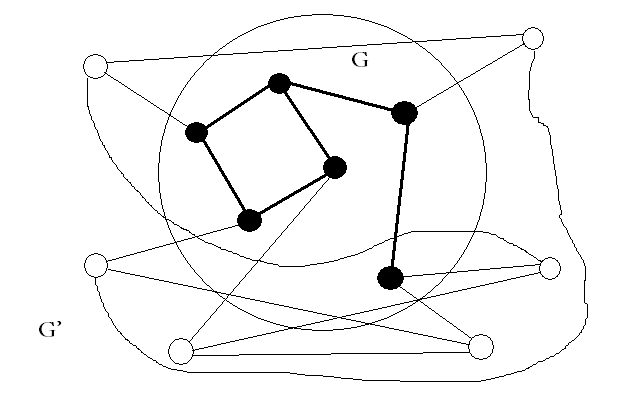
\includegraphics[scale=0.5]{regular.png}
\caption{constructed regular graph}
\end{center}
\end{figure}
Now it's time to prove the if and only if property. If there is a Vertex Cover in G, where $S \subseteq V$ and $|S| \le K$. We can easily know that $S^{'} = S \cup \{v|$ $v$ is added by construction $\}$ is also a vertex cover, because all the edges introduced by construction are covered by these vertices. Conversely, if there is a Vertex Cover $S^{'}$ in $G^{'}$, we can know that, the edges in $G$ can not be covered by the vertices added. So we can simply remove the vertices which is added by construction from $S^{'}$. Now in order to cover all the edges in $G$, the rest vertices in $S^{'}$ must be a Vertex Cover in $G$. \\
Then we proved that Vertex Cover problem remain NP-C when restricted to regular graphs.
\subsection{Does the VC problem remain NP-C when restricted to ring graphs?}
No, it belongs to polynomial class. \\
Actually ring graph is a special case of regular graph, with vertex degree 2. In this case given graph $G=(V,E)$, we know that if $|V|=N$, then $|E|=N$ too. Because each vertex has degree 2, in order to cover $N$ edges, it at least needs $\frac{N}{2}$ vertices. Without losing generality, assume the graph is connected like this $<(v_{1},v_{2}),(v_{2},v_{3}), ..., (v_{N-1},v_{N}),(v_{N},v_{1})>$. Then we can construct the vertex cover this way, pick up first vertex $v_{1}$, without choosing its neighbor, but choose its neighbor's neighbor, in this case $v_{3}$, repeat the same task on $v_{3}$, until reaching the ending vertex. If $N$ is even, the size of vertex cover is $\frac{N}{2}$, otherwise $\lceil{\frac{N}{2}}\rceil$. Of course all the vertices selected will cover all the edges in $G$. And it is related to the number of vertex in $G$, so it belongs to polynomial class.
\subsection{Does the VC problem remain NP-C when restricted to complete graphs?}
This one depends on the vertex degree. If the degree is 2, which means the graph is a triangle, according to the above prove, we know that it can be solved in polynomial time. \\
If the vertex degree is larger than 2, it is also a special case of regular graph, because all the vertices have the same degree $N-1$, where $N=|V|$. Apparently it remains NP-C. \\
\[VC_{complete} \in \left\{ 
\begin{array}{l l}
  P & \quad \mbox{if vertex degree $\le$ 2}\\
  NP-C & \quad \mbox{if vertex degree $\ge$ 3}\\ \end{array} \right. \]
\end{document}